\clearpage
\section{Turbo kódy}
\subsection{Uveďte a popište metody modifikace kódů.}
Nejběžnější metody modifikace kódů jsou: Zkracování kódů, rozšiřování kódů, děrování kódu, zvětšení kódu, zmenšení kódu, kombinování kódů a zřetězené kódy.
\begin{itemize}
    \item \textbf{Zkracování} - Princip zkrácení kódu spočívá ve zmenšení počtu využívaných kódových kombinací. Prvních $s$ prvků původního kódu je nulových a nepřenáší se - odstranění informačních prvků.
    \item \textbf{Rozšiřování} - Obecně rozšíření kódu spočívá v přidání $e$ zabezpečovacích prvků. Nejčastějším způsobem rozšiřování kódu je přidání paritního prvku
    \item \textbf{Děrování} - Děrování spočívá v odstraňování zabezpečovacích prvků, v Turbo kódech.
    \item \textbf{Zvětšení a zmenšení kódu} -  Vedou k nelineárním kódům. Zmenšování (zvětšování) kódu spočívá v odstranění (přidání) některých kódových slov z kódu.
    \item \textbf{Kombinování} - např. sčítat kódové kombinace různých kódů
    \item \textbf{Zřetězení} - také kombinování; výsledný zabezpečený datový tok z prvního kodéru je následně ještě jednou zabezpečen dalším kódem.
\end{itemize}

\subsection{Podrobněji vysvětlete metodu zkracování kódu.}
Je-li původní kód (n, k, d), vhodnou volbou celého čísla s v rozsahu $0 \leq s < k$ jej
zkrátíme na kód (n - s, k - s, ds), kde Hammingova vzdálenost zkráceného kódu ds je $ds \geq d$.
Vytvářecí matici zkráceného kódu Gs tvoří s+1 až k-tý řádek a s+1 až n-tý sloupec vytvářecí
matice G zkracovaného systematického lineárního blokového kódu. \\
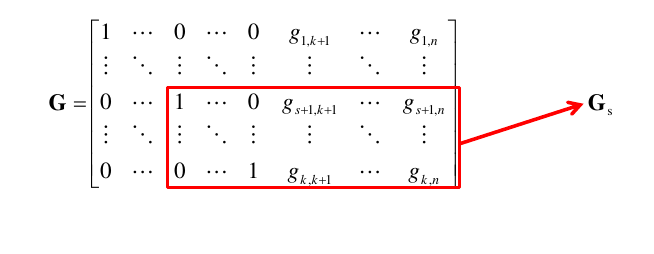
\includegraphics[width=16cm]{images/9_zkrac_obecne.png}\\
Např.: kód (7,4):\\
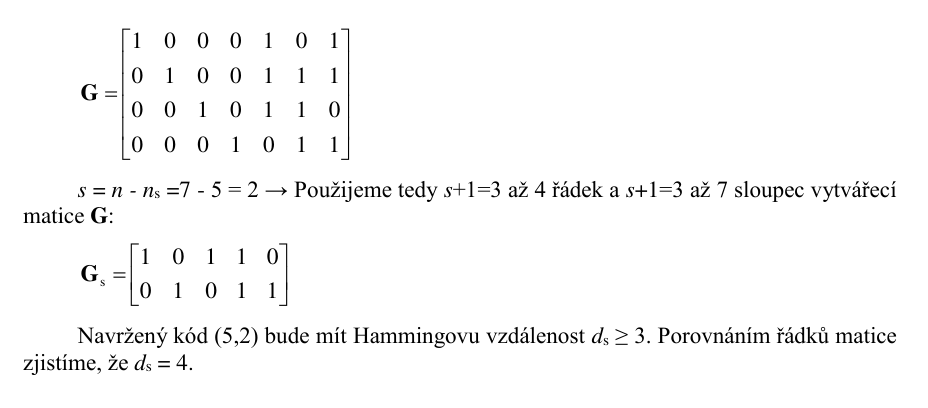
\includegraphics[width=16cm]{images/9_zkrac_priklad.png}

\subsection{Co specifikuje Hammingova hranice?}
\begin{itemize}
    \item Udává, kolik chyb je kód schopen opravit
    \item Počet syndromů, $2^{n-k}$ musí být větší nebo roven počtu kombinací chyb:
    $$2^{n-k}\geq \sum_{e=0}^t \binom{n}{e}$$
\end{itemize}

\subsection{Co je to prokládaní a proč se používá? Jaké znáte metody prokládaní?}
Je to metoda, která umožňuje změnou pořadí prvků dosáhnout změnu typu chyb ze shlukových na nezávislé. V minulosti hlavně u přenosu televizního obrazu z důvodu veliké potřebné šířky pásma (blikání). Nejběžnější \textbf{metody} prokládání jsou: Konvoluční prokládání a blokové prokládání.

\subsection{Co je to prokládání a proč se používá?}
\begin{itemize}
    \item interleaving
    \item Změna pořadí prvků -> změna shlukových chyb na nezávislé
\end{itemize}
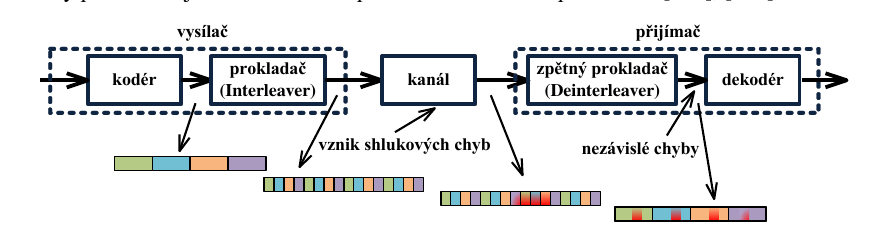
\includegraphics[width=16cm]{images/9_prokladani.png}

\subsection{Jaké znáte základní dvě metody prokládání?}
\begin{itemize}
    \item Blokové - do prokladače jdou bloky jako  řádku, z něj se čte po sloupcích
    \item konvoluční - trojúhelníkové pole zpožďovacích článků v prokladači a zpětném prokladači
    (každý další řádek má o 1 zpožďovací článek navíc, u zpětného naopak) \\
    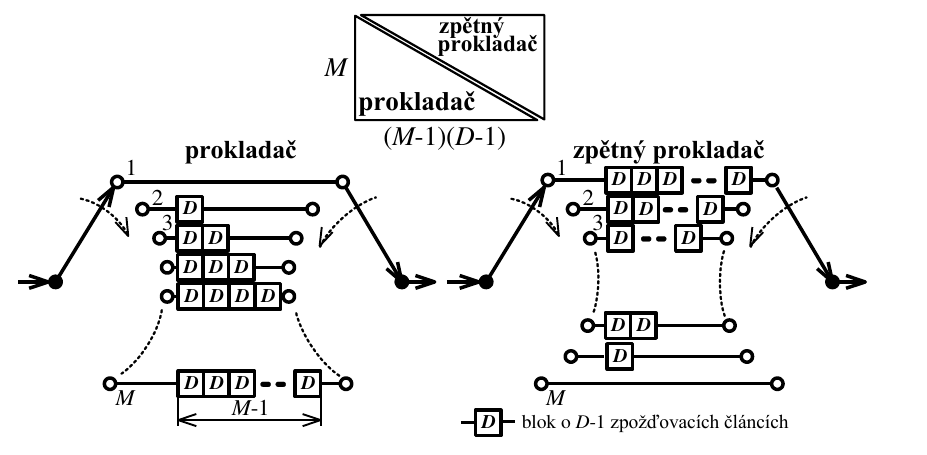
\includegraphics[width=16cm]{images/9_konvol_prokl.png}
\end{itemize}

\subsection{Co udává hloubka prokládání \textit{D}?}
Počet bloků účastnících se prokládání

\subsection{Co jsou to zřetězené kódy?}
\begin{itemize}
    \item výsledný zabezpečený datový tok z prvního kodéru je následně ještě jednou zabezpečen dalším kódem
    \item  Metoda se často kombinuje s prokládáním. Pro dekódování se vyžívaná modifikovaná Viterbiho metoda.
\end{itemize}

\subsection{Jaké dva základní typy zřetězení existují a jak se označují?}
\begin{itemize}
    \item paralelní zřetězení (turbo kódy)
    \item sériové zřetězení - násobné kódy (product code)
\end{itemize}

\subsection{Která technika se často využívá při zřetězení kódů?}
\begin{itemize}
    \item Metoda zřetězení se často kombinuje s prokládáním. Pro dekódování se vyžívaná modifikovaná Viterbiho metoda.
\end{itemize}

\subsection{Stručně vysvětlete princip měkkého dekódování algoritmem SOVA.}
\begin{itemize}
    \item Podobný Viterbiho algoritmu, používá mřížový diagram
    \item Určuje maximální akumulovanou pravděpodobnost pro každý stav místo ceny cesty
    \item Používá se proměnná $L_i$, která: $L_i=1$, pokud se shoduje v obou bitech,
    $L_i=0$ pokud v 1, $L_i=-1$ pokud v žádném
    \item Postupuje se od konce, zjistí se tvrdý výstup
    \item Celková pravděpodobnost každého stavu je součet pravděpodobnosti okamžitého stavu a apriorní pravděpodobnost,
    $L=L_i+L_p$
    \item Jsou brány v potaz také nepřežívající cesty, z nich je počítá funkce Delta (rozdíl hodnot L pro cesty), 
    z nich se tvoří měkký výstup
    \item Rozhodnutí se mění, pokud se mění bity
    \item Hodnoty funkce Delta jsou měkkým výstupem, upraví se koeficientem spolehlivosti kanálu
    \item První dekodér získá systematická data, druhý kodér získá kódovou informaci, která se předá druhému 
    dekodéru a takto iterujeme, záleží na implementaci, nakonec je kladným hodnotám přiřazen bit 1, záporným 0
\end{itemize}
